%%
%% NuSTAR paper formatted for ACM Multimedia (ACM MM)
%% Uses acmart sigconf template.
%% Requires acmart.cls and ACM-Reference-Format.bst (copy from ACMMM/ folder).
%%

\documentclass[sigconf, screen, review, anonymous]{acmart}

\AtBeginDocument{%
  \providecommand\BibTeX{{%
    Bib\TeX}}}

%% Rights management information (update with actual values upon acceptance)
\setcopyright{acmlicensed}
\copyrightyear{2026}
\acmYear{2026}
\acmDOI{XXXXXXX.XXXXXXX}
\acmConference[MM '26]{ACM Multimedia 2026}{October 2026}{Melbourne, Australia}
\acmISBN{978-1-4503-XXXX-X/2026/10}

% Recommended, but optional, packages for figures and better typesetting:
\usepackage{microtype}
\usepackage{graphicx}
\usepackage{booktabs}   % for professional tables

% For theorems and such
\usepackage{amsmath}
\usepackage{mathtools}
\usepackage{amsthm}
\usepackage{float}

% Other packages from your original IJCAI file
\usepackage{multirow}
\usepackage{xcolor}
\usepackage{colortbl}
\usepackage{placeins} % Keep floats within sections
\definecolor{dodgerblue}{rgb}{0.12, 0.56, 1.0}
\definecolor{graybg}{gray}{0.95}

% if you use cleveref..
\usepackage[capitalize,noabbrev]{cleveref}

% Algorithm packages
\usepackage{algorithm}
\usepackage{algorithmic}

%%%%%%%%%%%%%%%%%%%%%%%%%%%%%%%%
% THEOREMS
%%%%%%%%%%%%%%%%%%%%%%%%%%%%%%%%
\theoremstyle{plain}
\newtheorem{theorem}{Theorem}[section]
\newtheorem{proposition}[theorem]{Proposition}
\newtheorem{lemma}[theorem]{Lemma}
\newtheorem{corollary}[theorem]{Corollary}
\theoremstyle{definition}
\newtheorem{definition}[theorem]{Definition}
\newtheorem{assumption}[theorem]{Assumption}
\theoremstyle{remark}
\newtheorem{remark}[theorem]{Remark}
\newtheorem{example}{Example}

\begin{document}

\title[NuSTAR: Robust Test-Time Adaptation via Stochastic Smooth Adversarial Warping]{NuSTAR: Robust Test-Time Adaptation via Stochastic Smooth Adversarial Warping}

\author{First Author}
\authornote{Both authors contributed equally to this research.}
\email{first.author@institution.edu}
\affiliation{%
	\department{Department of XXX}
	\institution{University of YYY}
	\city{Location}
	\country{Country}
}

\author{Second Author}
\authornotemark[1]
\email{second.author@institution.edu}
\affiliation{%
  \department{Department of XXX}
  \institution{University of YYY}
  \city{Location}
  \country{Country}
}
\affiliation{%
  \institution{Company Name}
  \city{Location}
  \country{Country}
}

\author{Third Author}
\affiliation{%
  \institution{Company Name}
  \city{Location}
  \country{Country}
}

\renewcommand{\shortauthors}{First Author et al.}

\begin{abstract}
	Source-free test-time adaptation (TTA) for time-series streams is often driven by entropy minimization, which can be brittle when the stream contains natural structural corruptions. In real deployments, transient artifacts and low-SNR segments can yield confident predictions with little semantic content, and online updates then amplify the error. We propose \textbf{NuSTAR}, an online SF-TTA framework that is designed for this setting. NuSTAR uses \textbf{Stochastic Smooth Adversarial Warping (SSAW)} to generate an adversarial second view by searching a low-dimensional cubic-spline amplitude scaling space under a bounded safety corridor; the search is implemented as a one-shot, gradient-free selection suitable for streaming inference. To prevent contaminated samples from driving updates, a \textbf{Triple-Safe Reliability Gate} filters samples using (i) a robust quantile-based entropy threshold, (ii) prototype-based semantic alignment, and (iii) raw--perturbed consistency. Updates are restricted to samples passing all three criteria, preventing self-reinforcing degradation under structural corruption. On Sleep-EDF, UCI-HAR, and MFD (five shifts each), NuSTAR improves Macro-F1 over strong SF-TTA baselines and remains stable on high-noise shifts (e.g., +5.38 on Sleep-EDF and +4.46 on UCI-HAR under a fixed-source protocol).
\end{abstract}

%%
%% CCS Concepts -- generate your own at https://dl.acm.org/ccs/ccs.cfm
%%
\begin{CCSXML}
<ccs2012>
 <concept>
  <concept_id>10010147.10010178.10010187</concept_id>
  <concept_desc>Computing methodologies~Machine learning</concept_desc>
  <concept_significance>500</concept_significance>
 </concept>
 <concept>
  <concept_id>10010147.10010178.10010224</concept_id>
  <concept_desc>Computing methodologies~Neural networks</concept_desc>
  <concept_significance>300</concept_significance>
 </concept>
 <concept>
  <concept_id>10010147.10010257.10010258.10010259</concept_id>
  <concept_desc>Computing methodologies~Unsupervised learning</concept_desc>
  <concept_significance>300</concept_significance>
 </concept>
</ccs2012>
\end{CCSXML}

\ccsdesc[500]{Computing methodologies~Machine learning}
\ccsdesc[300]{Computing methodologies~Neural networks}
\ccsdesc[300]{Computing methodologies~Unsupervised learning}

\keywords{Test-Time Adaptation, Time Series, Active Search, Robustness}

\maketitle

	% ========================================================
	% 1. Introduction
	% ========================================================
\section{Introduction}
\label{sec:intro}

Deep learning models for time series analysis achieve strong performance
under controlled conditions, but degrade in deployment when the test
distribution diverges from training. In sensor-based systems, this
divergence is both common and unpredictable: physical wear, environmental
interference, and changing operating conditions continuously alter the
statistics of incoming data \citep{wu2023timesnet,yue2022ts2vec}.
Source-Free Test-Time Adaptation (SF-TTA) addresses this by adapting a
pretrained model online using only unlabeled target samples, without
revisiting the source data \citep{liang2020shot}.

The dominant approach in online SF-TTA is entropy minimization. TENT
\citep{wang2021tent} updates normalization parameters to reduce prediction
entropy on the test stream; SAR \citep{niu2023sar} adds selective
filtering to avoid updates when gradients are unreliable; CoTTA
\citep{wang2022cotta} enforces consistency between a student and an
exponential-moving-average teacher across stochastically augmented views.
These methods share a common assumption: that test inputs, however shifted,
still carry valid semantic content. Under this assumption, low entropy
indicates a confident and correct prediction, and entropy minimization
provides a reliable self-supervised signal.

This assumption fails in a class of corruption that is common in physical
sensor streams but largely absent from vision benchmarks: Natural Structural
Corruption. Unlike visual distribution shifts (e.g., weather or lighting
changes) that alter appearance while preserving object identity, sensor
faults alter the signal's information content. Signal freezing, impedance
drift, and sensor blackout \citep{lai2021revisiting, darban2023deep} can
suppress semantic information entirely, leaving extended segments of the
stream non-informative. Under these conditions, entropy minimization becomes
ill-posed. Corrupted inputs frequently trigger the Over-Certainty
Phenomenon \citep{amin2025overcertaintyphenomenonmoderntesttime}: networks
assign high confidence to semantically meaningless patterns because
structural artifacts activate convolutional filters strongly
\citep{nguyen2015deepneuralnetworkseasily}. Confidence-based filters then
admit these corrupted samples, self-confirming updates amplify the error,
and the model collapses \citep{gong2023sotta}. Standard augmentations
compound the problem: generic perturbations such as additive noise and
random jitter do not emulate sensor faults and therefore fail to expose
the model's most vulnerable decision regions during adaptation.

Addressing this requires two capabilities that existing methods lack.
First, a mechanism to actively probe the model with physically plausible
structural perturbations, so that adaptation is driven by worst-case
realistic shifts rather than generic noise. Second, a reliable filter that
blocks updates when the self-supervised signal cannot be trusted---one that
goes beyond entropy thresholding, which is precisely what fails under
structural corruption.

We propose \textbf{NuSTAR}, a source-free online TTA framework built
around these two capabilities. \textbf{Stochastic Smooth Adversarial Warping (SSAW)} parameterizes perturbations on a low-dimensional
cubic-spline manifold, searching for the worst-case amplitude drift within
a bounded safety corridor in a single gradient-free forward pass. The
spline constraint restricts perturbations to smooth, globally structured
deformations consistent with gradual sensor degradation, avoiding the
high-frequency artifacts that PGD-style attacks introduce. Spectral analysis
confirming this property is provided in Appendix~\ref{app:ssaw}.
A \textbf{Triple-Safe Reliability Gate} then determines which samples are
safe to learn from, combining a quantile-based entropy check robust to
transient bursts, a prototype alignment check that detects confident-but-
semantically-invalid inputs, and a cross-view consistency check that
exploits the SSAW perturbation directly.

\textbf{Contributions.} Our main contributions are as follows:

\begin{itemize}
	\item \textbf{Problem setting and failure analysis.}
	We characterize Natural Structural Corruptions in streaming
	time-series TTA---including sensor blackouts, impedance drift, and
	signal freezing---as a class of structure-altering failures that
	violate the label-preserving assumption of standard entropy
	minimization. We show empirically that such corruptions induce
	over-confident adaptation dynamics, leading to harmful self-training
	loops and progressive performance degradation.

	\item \textbf{Physically plausible adversarial augmentation (SSAW).}
	We propose Stochastic Smooth Adversarial Warping, a gradient-free
	adversarial augmentation scheme that searches a low-dimensional spline
	manifold for worst-case amplitude drifts. SSAW generates physically
	realistic perturbations suitable for streaming inference and provides
	an informative consistency signal for the reliability gate.

	\item \textbf{Safe online updating.}
	We introduce a Triple-Safe Reliability Gate that combines statistical,
	semantic, and consistency criteria to decide \emph{when} to update,
	preventing self-reinforcing degradation under structural corruption.

	\item \textbf{Empirical evaluation.}
	On Sleep-EDF, UCI-HAR, and MFD under a unified fixed-source protocol,
	NuSTAR achieves the highest average Macro-F1 across all datasets,
	outperforming the strongest baselines by +5.38 on Sleep-EDF (over
	ACCUP) and +4.46 on UCI-HAR (over TENT).
\end{itemize}


% ========================================================
% 2. Related Work
% ========================================================
\section{Related Work}
\label{sec:related}

\subsection{Problem setting and taxonomy of test-time adaptation}
Adaptation under distribution shift has long been studied in Unsupervised Domain Adaptation (UDA) \citep{ganin2016domain, long2015learning}, where source-domain data are available, and models are aligned across domains. Source-Free Test-Time Adaptation (SF-TTA) \citep{liang2020shot} removes access to source data and adapts a pretrained model at deployment using only unlabeled target samples.

We study online TTA, where samples arrive sequentially and the model updates without storing past data. Compared with continual adaptation work that mainly tracks gradual drift under preserved label semantics, we consider a noisier regime in which Natural Structural Corruptions may contaminate the stream, such as sensor failures \citep{sunesh2026modeling}. In this setting, the main difficulty is not only distribution mismatch but also deciding which test inputs provide a usable self-supervision signal; structure-altering outliers can slip into the update loop and amplify errors over time.


\subsection{The entropy and self-training lineage}
Many online TTA methods rely on prediction confidence for self-supervision. TENT \citep{wang2021tent} minimizes prediction entropy on unlabeled target data and limits adaptation to normalization parameters. Building on this idea, EATA \citep{niu2022eata} and SAR \citep{niu2023sar} add safeguards and update selectively when the self-supervision signal appears trustworthy.

These assumptions can break under structural corruption. During sensor failures such as signal freezing or disconnection, models may exhibit the Over-Certainty Phenomenon \citep{amin2025overcertaintyphenomenonmoderntesttime}, assigning high confidence to semantically invalid inputs. In this case, confidence-driven filters may admit corrupted samples, and subsequent updates can compound errors and accelerate degradation \citep{gong2023sotta}.

\subsection{Consistency-based and time-series-specific adaptation}
CoTTA \citep{wang2022cotta} maintains a teacher model as an exponential moving average of the student and enforces prediction consistency across stochastically augmented views, while EcoTTA \citep{song2023ecotta} reduces its memory and compute overhead. For time-series specifically, NOTE \citep{gong2022note} uses prediction-balanced sampling to address temporally correlated shifts, Raincoat \citep{he2023domain} aligns spectral features to disentangle frequency-band drift, and ACCUP \citep{gong2025accup} introduces uncertainty-aware prototyping over shifted representations.

Despite their differences, these methods share a common assumption that each test window remains structurally informative. The stochastic augmentations used in consistency frameworks are not designed to emulate sensor failures, and time-series temporal constraints can reinforce corrupted trends when collective anomalies \citep{lai2021revisiting} or information blackouts \citep{sunesh2026modeling} contaminate the stream.

\subsection{Adversarial augmentation and physical plausibility}
Augmentation-based self-supervision in online TTA relies on approximately label-preserving transformations \citep{chen2020simple}. Random augmentations, as in CoTTA, provide a generic consistency signal but are agnostic to the model's failure modes. This gap motivates augmentation schemes that actively probe for vulnerabilities rather than relying solely on stochastic perturbations.

Adversarial augmentation builds challenging views that stress the current model. Directly applying standard image attacks such as PGD \citep{madry2018towards} to time-series can be problematic: unconstrained gradient perturbations often introduce high-frequency sawtooth artifacts that are physically implausible for continuous systems with inertia \citep{tu2020physically,pialla2025time}. Adapting to such artifacts risks learning unrealistic patterns that transfer poorly to genuine sensor drifts.
Recent work, therefore, emphasizes adversarial perturbations that remain smooth, low-dimensional, and physically plausible. Smooth and approximately invertible warping families \citep{demirel2025shifting} better match realistic mechanism drifts and allow adversarial augmentation to emulate gradual degradation rather than injecting arbitrary noise. NuSTAR addresses these weakness by Stochastic Smooth Adversarial Warping(SSAW), which constrains adversarial search to a spline manifold, combining it with a triple safe gate that blocks updates when the self-supervised signal cannot be trusted.


	% ========================================================
	% 3. Methodology
	% ========================================================
\section{Methodology}
\label{sec:method}

Real-world time series streams exhibit two distinct forms of non-stationarity: gradual physical drift (low-frequency), arising from sensor aging or electrolyte drying, which manifests as continuous distributional shifts; and transient noise bursts (high-frequency), caused by sudden artifacts or loose contacts. Existing TTA methods tend to fail at one end or the other: over-adaptation corrupts the model when transient bursts arrive, while conservative filtering fails to track gradual drifts.

NuSTAR is designed to handle both. As illustrated in Figure~\ref{fig:framework}, it operates on two levels: SSAW (Sec.~\ref{sec:ssaw}) actively simulates smooth physical drifts to generate informative adversarial views, and the Triple-Safe Reliability Gate (Sec.~\ref{sec:gate}) blocks unreliable updates from transient bursts. The optimization objective is described in Sec.~\ref{sec:optimization}.

	\subsection{Overview and problem definition}
	\label{sec:overview}

	% === [INSERTED] Model Architecture Figure ===
	\begin{figure*}[t]
		\vskip 0.2in
		\centering
		\includegraphics[width=0.98\textwidth]{diagram.pdf}
		\caption{\textbf{The overall framework of NuSTAR.} Given a streaming time series input, NuSTAR first generates a dual-view representation via Stochastic Smooth Adversarial Warping (SSAW) (Sec.~\ref{sec:ssaw}). It then applies the Triple-Safe Reliability Gate (Sec.~\ref{sec:gate}) to block unreliable gradients through statistical, semantic, and consistency checks.Only if the input data passes the three checks can it enter the $\mathcal{D}_{active}$}
		\label{fig:framework}
	\end{figure*}

	\begin{figure}[t]
		\vskip 0.2in
		\centering
		\includegraphics[width=0.85\linewidth]{rms_shift_EEG_12_to_5.pdf}
		\caption{\textbf{Motivation for smooth amplitude warping.} Distribution of signal RMS (energy) on the EEG dataset (scenario $12 \to 5$). The target domain (red) shows a global amplitude shift of $\Delta \mu \approx +26\%$ relative to the source (blue), motivating smooth amplitude warping as a physically grounded augmentation strategy.}
		\label{fig:rms_shift}
	\end{figure}
	% ============================================

We focus on source-free test-time adaptation. Let $f_{\theta}$ denote an encoder and $h_{\phi}$ a classifier, pretrained on a source domain $\mathcal{D}_S$. At test time, the model receives a stream of unlabeled time series $\mathcal{X}_{test} = \{x_t\}_{t=1}^N$, where samples arrive sequentially and cannot be revisited. The goal is to adapt $\theta, \phi$ online to minimize error on the drifting target domain while preventing collapse caused by corrupted samples.

\subsection{Stochastic Smooth Adversarial Warping (SSAW)}
\label{sec:ssaw}

\textbf{Motivation.}
Adversarial augmentation methods designed for computer vision, such as PGD, optimize perturbations in pixel space and produce high-frequency additive noise. This is a poor fit for physical sensor streams, where intrinsic system drifts (sensor aging, impedance changes) are inherently low-frequency while high-frequency components correspond to external noise such as electromagnetic interference. Applying PGD-style perturbations to time series forces the model to overfit to unrealistic artifacts rather than the structural corruptions that appear in practice.

We instead seek perturbations that are smooth and globally structured, consistent with gradual sensor degradation, while still finding the worst-case view for the current model.

\begin{figure}[t]
	\vskip 0.1in
	\centering
	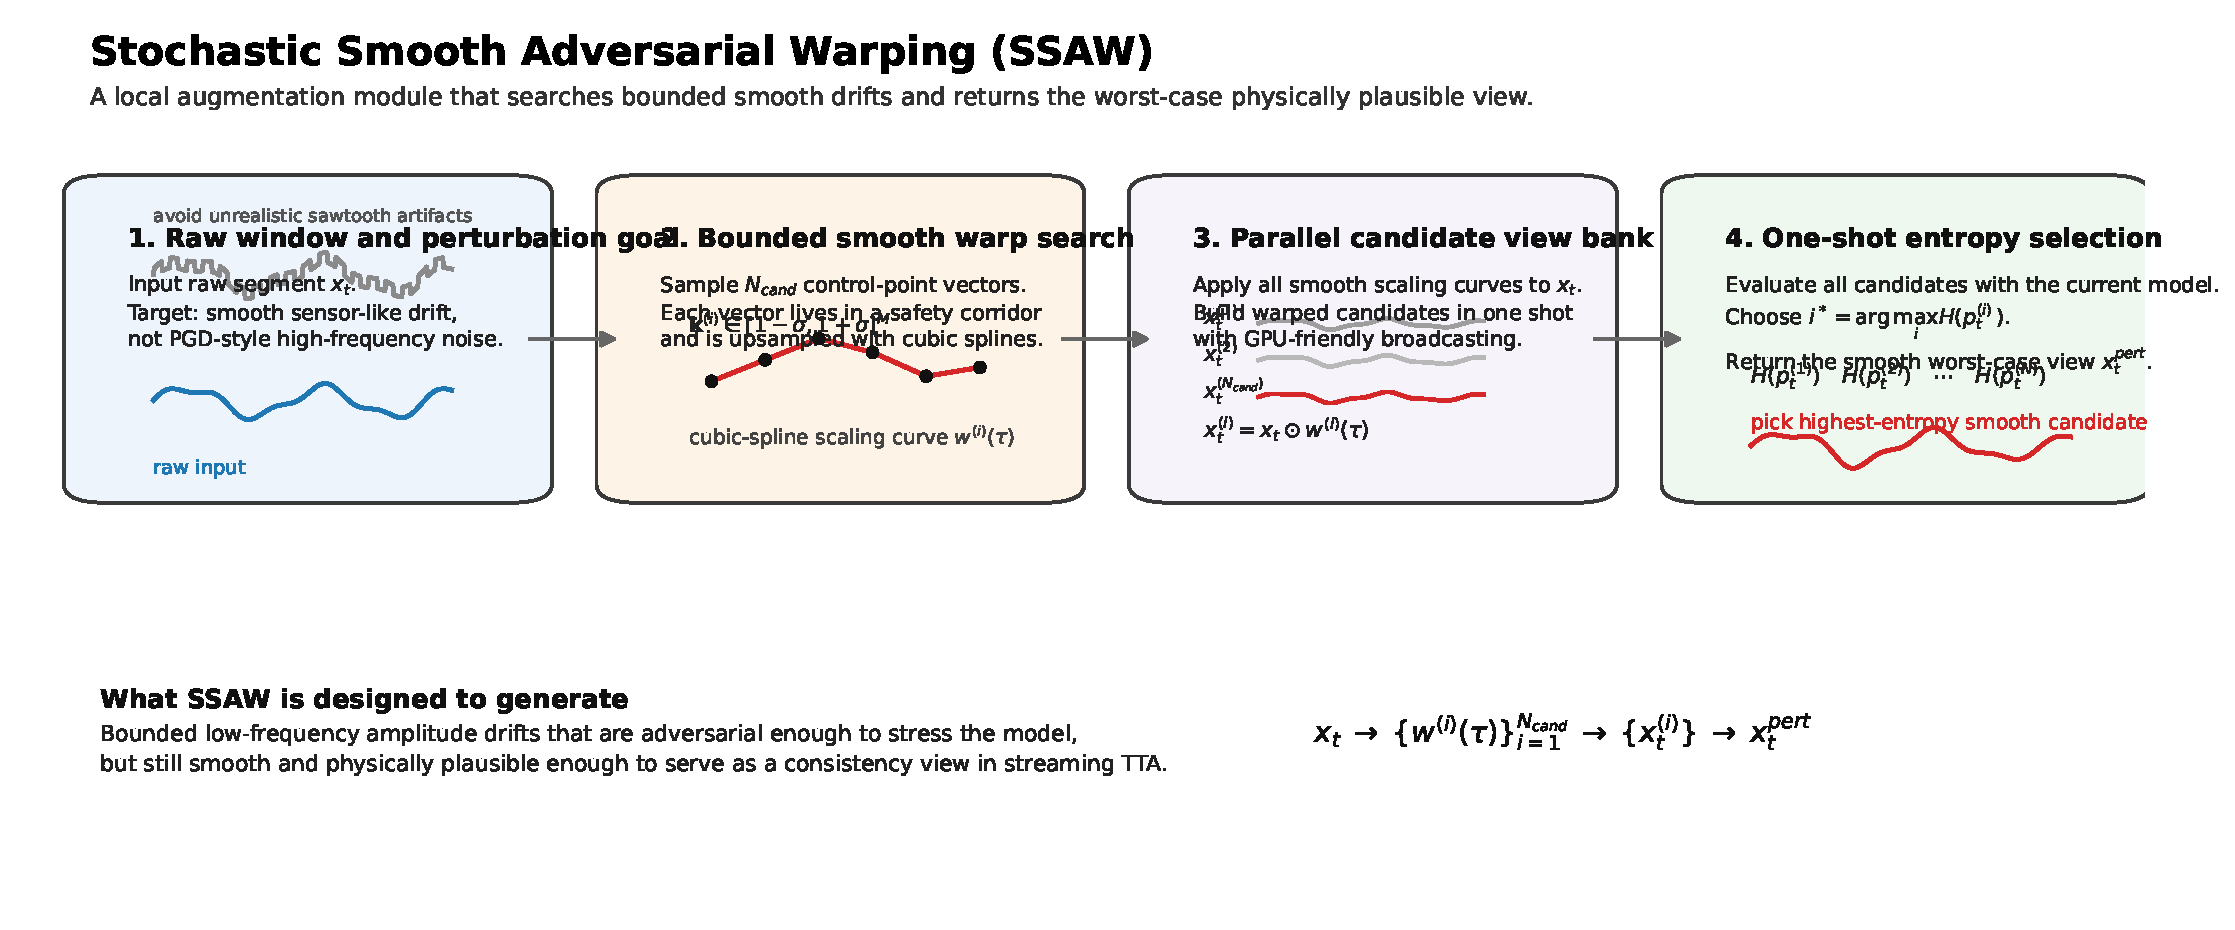
\includegraphics[width=\columnwidth]{ssaw_module_diagram.pdf}
	\caption{\textbf{SSAW submodule illustration.} SSAW starts from a raw input window $x_t$, samples bounded amplitude control points, interpolates them into smooth cubic-spline scaling curves, and forms a bank of warped candidate views. A one-shot entropy evaluation then selects the highest-entropy candidate as the smooth worst-case view $x_t^{pert}$, which is passed to the consistency branch and reliability gate.}
	\label{fig:ssaw_module}
\end{figure}

\textbf{From high-dim to low-dim.}
Given an input time series $x \in \mathbb{R}^{C \times L}$, directly optimizing a perturbation vector of length $L$ introduces excessive degrees of freedom and risks generating high-frequency noise. We instead model sensor drift as a continuous amplitude scaling curve $w(\tau)$ defined by $M$ sparse control points $\mathbf{k} = \{k_j\}_{j=1}^M$ uniformly spaced over the temporal dimension. Enforcing $M \ll L$ (e.g., $M=10$ for $L=3000$) acts as a low-pass filter, restricting optimization to global structural changes and preventing local high-frequency anomalies.

\textbf{Cubic spline interpolation.}
We map the discrete control points $\mathbf{k}$ to the continuous curve $w(\tau)$ via cubic spline interpolation. Natural cubic splines minimize the bending energy $E[w] = \int \|w''(\tau)\|^2 d\tau$ \citep{deboor1978practical}, penalizing high-frequency complexity and keeping generated drifts within the manifold of physically plausible sensor degradation. $C^2$-continuity also provides a differentiable trajectory for gradient estimation \citep{durkan2019neural,kidger2020neural}, avoiding instabilities from non-differentiable cusps.

Linear interpolation introduces $C^0$ discontinuities at control points, producing sawtooth artifacts inconsistent with smooth sensor degradation. Higher-order polynomials introduce spurious oscillations between control points (Runge's phenomenon \citep{unser1999splines}), injecting high-frequency components that violate the low-frequency constraint. Natural cubic splines avoid both failure modes, making them the appropriate basis for physically-constrained adversarial search.

	\textbf{Micro-warping.}
	While smoothness ensures physical plausibility, unbounded amplitude scaling can still destroy semantic information (e.g., scaling a signal to zero). We constrain each control point $k_j$ to the interval $[1-\epsilon, 1+\epsilon]$ (e.g., $\epsilon=0.15$), modeling multiplicative sensitivity drift without identity-changing distortions. Within this safety corridor $\Omega$, we search for the configuration $\mathbf{k}^*$ that maximizes prediction entropy:
	\begin{equation}
		\mathbf{k}^* = \arg\max_{\mathbf{k} \in \Omega} H\left( \sigma(h_\phi(f_\theta(x \odot 	w(\tau; \mathbf{k})))) \right).
		\label{eq:adv_attack}
	\end{equation}

\textbf{Gradient-free parallel sampling.}
PGD-style iterative backpropagation is prohibitively expensive for real-time streams. Instead, we exploit the low dimensionality of $\mathbf{k}$ to search via parallel sampling with GPU vectorization, completing the entire search in a single forward pass under \texttt{torch.no\_grad()}.

The procedure has three steps. First, we simultaneously sample $N_{cand}$ (e.g., 16) candidate control point vectors from $\Omega$ and upsample each via cubic splines, yielding a tensor of drift curves $\mathbf{W} \in \mathbb{R}^{N_{cand} \times 1 \times 1 \times L}$. Second, using tensor broadcasting, we apply all candidates to the mini-batch to form a super-batch of shape $[(N_{cand} \cdot B) \times C \times L]$. Third, a single forward pass evaluates all candidates, and we select the one maximizing batch-averaged entropy:
\begin{equation}
	\begin{split}
		\mathbf{k}^* &= \mathbf{k}^{(n^*)} \quad \text{s.t.}, \\
		n^* &= \arg\max_{n \in \{1..N_{cand}\}} \underbrace{\frac{1}{B} \sum_{i=1}^B \mathbf{E}_{n,i}}_{\text{Batch-averaged entropy}}.
	\end{split}
\end{equation}
This reduces computational complexity from $O(L \cdot \text{Steps})$ to $O(1)$ relative to optimization steps.

	\textbf{Dual-branch formulation.}
	The model processes each mini-batch under both the raw view $x_t$ and the selected worst-case view $x^{pert}_t = x_t \odot w(\tau; \mathbf{k}^*)$:
	\begin{equation}
	\begin{aligned}
		z^{raw}_t &= f_{\theta}(x_t), \quad &p^{raw}_t &= \sigma(h_{\phi}(z^{raw}_t)), \\
		z^{pert}_t &= f_{\theta}(x^{pert}_t), \quad &p^{pert}_t &= \sigma(h_{\phi}(z^{pert}_t)).
	\end{aligned}
	\label{eq:dual_branch}
	\end{equation}
	The ensemble $\bar{p}_t = (p^{raw}_t + p^{pert}_t)/2$ is used in subsequent reliability gating.



	% === Algorithm 1 ===
\begin{algorithm}[tb]
	\caption{\textbf{NuSTAR}: Online Test-Time Adaptation via Active Purification}
	\label{alg:nustar}
	\begin{algorithmic}[1]
		\REQUIRE Pre-trained model $f_{\theta}, h_{\phi}$; Stream $\mathcal{X}_{test}$.
		\REQUIRE Hyperparams: Warping intensity $\sigma$, Quantile $\alpha$, Warm-up $N_{min}$, Sem-thresh $\delta_{sem}$, Cons-thresh $\gamma_{cons}$, Relax-rate $\lambda_{relax}$, Min-batch $\tau_{min}$.
		
		\STATE \textbf{Initialization:}
		\STATE \quad Load source anchors: \textbf{L2-normalized} Classifier Weights (as initial Prototypes $\mathcal{M}$).
		\STATE \quad Initialize \textbf{FIFO History Window} $\mathcal{H} \leftarrow \emptyset$.
		
		\WHILE{test stream continues}
		\STATE Receive mini-batch $x_t$.
		
		\STATE \textbf{// 1. Stochastic Smooth Adversarial Warping (SSAW) (Sec. \ref{sec:ssaw})}
		\STATE Find worst-case control points $\mathbf{k}^*$ via Eq.~\ref{eq:adv_attack} (maximizing entropy).
		\STATE Generate perturbed view: $x^{pert}_t \leftarrow x_t \odot w(\tau; \mathbf{k}^*)$.
		\STATE Compute predictions: $p^{raw}, p^{pert}$ and ensemble $\bar{p}$.
		
		\STATE \textbf{// 2. Dynamic Thresholding via History Window}
		\IF{$|\mathcal{H}| < N_{min}$}
		\STATE $E_{th} \leftarrow \ln C$ \COMMENT{Cold start: max entropy}
		\ELSE
		\STATE $E_{th} \leftarrow \text{Quantile}(\mathcal{H}, \alpha)$ \COMMENT{Adaptive threshold}
		\ENDIF
		
		\STATE \textbf{// 3. Triple-Safe Gate with Relaxation (Sec. \ref{sec:gate})}
		\STATE Calculate masks: $\mathcal{C}_{stat}, \mathcal{C}_{sem}, \mathcal{C}_{cons}$.
		\STATE Active subset: $\mathcal{D}_{active} = \{x_i \mid \mathcal{C}_{stat} \wedge \mathcal{C}_{sem} \wedge \mathcal{C}_{cons}\}$.
		
		\IF{$|\mathcal{D}_{active}| < \tau_{min}$}
		\STATE $E_{th} \leftarrow E_{th} \cdot (1 + \lambda_{relax})$ \COMMENT{Safety Fallback}
		\STATE Re-calculate $\mathcal{D}_{active}$ with relaxed $E_{th}$.
		\ENDIF
		
		\STATE \textbf{// 4. Optimization (Sec. \ref{sec:optimization})}
		\IF{$|\mathcal{D}_{active}| > 0$}
		\STATE $\mathcal{L}_{total} = \text{ReweightedEntropy}(\mathcal{D}_{active})$.
		\STATE Update $\theta$ to minimize $\mathcal{L}_{total}$.
		\ENDIF
		
		\STATE \textbf{// 5. State Update}
		\STATE Update History: $\mathcal{H} \leftarrow \mathcal{H} \cup \{H(\bar{p}_i)\}_{\forall i}$.
		\STATE Update Prototypes $\mathcal{M}$ via \textbf{Quality-Aware EMA} using $z^{raw}$.
		\ENDWHILE
	\end{algorithmic}
\end{algorithm}

\subsection{Triple-Safe Reliability Gate}
\label{sec:gate}

Adapting to all incoming samples without filtering risks model collapse under structural corruption. We design a three-criterion filtering system to determine which samples are safe to use for parameter updates.


\textbf{Temporal ordering.}
Adaptation is a closed loop: the gate uses prototypes to decide which samples update those same prototypes. We resolve this by enforcing strict temporal ordering. At step $t$, gating decisions use the prototypes $\mu^{(t-1)}$ from the previous step. Only samples that pass the gate are eligible to update the prototypes to $\mu^{(t)}$, ensuring the prototype bank is never corrupted by samples it has not yet screened.

We accept a sample ($a_i = 1$) only if it passes all three checks:
\begin{equation}
	a_i = \mathbb{I}\left( \mathcal{C}_{stat} \right) \cdot \mathbb{I}\left( \mathcal{C}_{sem} \right) \cdot \mathbb{I}\left( \mathcal{C}_{cons} \right).
	\label{eq:triple_gate}
\end{equation}

\textbf{1. Statistical gate ($\mathcal{C}_{stat}$).}
A static entropy threshold is insufficient for non-stationary streams. A moving-average threshold ($\mu + \sigma$) is skewed by transient noise bursts with very high entropy, inflating the threshold and subsequently admitting corrupted samples.

We instead maintain a FIFO history window $\mathcal{H}_t = \{H(p_{t-N}), \dots, H(p_{t-1})\}$ and set the dynamic threshold $E_{th}(t)$ as a quantile:
\begin{equation}
	E_{th}(t) = \begin{cases}
		\ln C, & \text{if } |\mathcal{H}| < N \text{ (warm-up)} \\
		\text{Quantile}(\mathcal{H}, \alpha), & \text{otherwise}.
	\end{cases}
\end{equation}
Unlike the mean, quantiles are robust to outliers \citep{huber1981robust}: a single burst with $H=5.0$ in a queue of low-entropy samples does not shift the 70th percentile. Dynamic quantile adjustment also handles temporal distribution shifts without distributional assumptions \citep{gibbs2021adaptive}.


	\textbf{Quality-aware prototype update.}
	To provide a stable reference for the semantic gate, we maintain class prototypes $\mathcal{M}^{(t)} = \{\mu_1^{(t)}, \dots, \mu_C^{(t)}\}$ updated only from accepted samples. Let $\mathcal{S}_c = \{i \mid x_i \in \mathcal{D}_{active}, \hat{y}_i = c\}$ be the accepted samples predicted as class $c$. We compute a quality-weighted batch center using L2-normalized features $\hat{z}_i = z^{raw}_i / \|z^{raw}_i\|_2$:
	\begin{equation}
		\bar{\mu}_c = \sum_{i \in \mathcal{S}_c} \underbrace{\left( \frac{q_i}{\sum_{j \in \mathcal{S}_c} q_j} \right)}_{\text{Normalized weight } \omega_i} \cdot \hat{z}_i,
	\end{equation}
	where $q_i = 1 - H(p^{raw}_i)/\ln C$ maps prediction uncertainty to a weight in $[0,1]$: a zero-entropy sample gets $q=1$ and a maximally uncertain sample gets $q=0$. If $\mathcal{S}_c = \emptyset$, the update for class $c$ is skipped. The global prototype is then updated via EMA and re-projected onto the unit hypersphere:
	\begin{equation}
		\begin{aligned}
		\tilde{\mu}_c^{(t)} &= \eta \cdot \mu_c^{(t-1)} + (1 - \eta) \cdot \bar{\mu}_c, \\
		\mu_c^{(t)} &= \frac{\tilde{\mu}_c^{(t)}}{\|\tilde{\mu}_c^{(t)}\|_2}.
		\end{aligned}
		\label{eq:proto_ema}
	\end{equation}

	\textbf{2. Semantic gate ($\mathcal{C}_{sem}$).}
	Statistical filtering alone cannot catch confidence mimicry, where high-amplitude artifacts produce low-entropy predictions. This occurs because convolutional networks are sensitive to high-frequency features \citep{wang2020high}: sharp edges and repetitive spikes act as super-stimuli for specific filters, triggering extreme softmax activations. Recent work on robust TTA confirms that such outliers can hijack adaptation by masquerading as confident samples \citep{park2024medbn}. Since entropy cannot distinguish genuine confidence from artifact overfitting, we add a check based on feature-space geometry.

	We require that an accepted sample's feature $z^{raw}_t$ aligns with the prototype of its predicted class. Samples that are confident but far from the cluster center are rejected:
	\begin{equation}
		\mathcal{C}_{sem}: \cos(z^{raw}_t, \mu_{\hat{y}}^{(t-1)}) \ge \delta_{sem}.
	\end{equation}

	\textbf{3. Consistency gate ($\mathcal{C}_{cons}$).}
	Since SSAW generates the worst-case physical shift, a reliably classified sample should remain stable under this perturbation. Samples whose predictions diverge significantly are rejected:
	\begin{equation}
		\mathcal{C}_{cons}: \text{KL}(p^{raw}_t \| p^{pert}_t) \le \gamma_{cons}.
	\end{equation}

	\textbf{Self-adaptive relaxation.}
	Strict gating can cause adaptation starvation during severe distribution shifts. If the accepted set $|\mathcal{D}_{active}|$ falls below a minimum threshold $\tau_{min}$, we temporarily relax the statistical threshold: $E_{th}' = E_{th} \cdot (1 + \lambda_{relax})$, then recompute $\mathcal{D}_{active}$.

\subsection{Optimization Objective}
\label{sec:optimization}

The total loss at step $t$ applies asymmetric reweighting over the
accepted subset $\mathcal{D}_{active}$:
\begin{equation}
	\mathcal{L}_{total}(t)
	=
	\frac{1}{|\mathcal{D}_{\mathrm{active}}|}
	\sum_{i \in \mathcal{D}_{\mathrm{active}}}
	\underbrace{\exp(E_{th} - H(\bar{p}_i))}_{\text{Reliability weight } \omega_i} \cdot
	H\!\left(p^{\mathrm{pert}}_i\right).
	\label{eq:total_objective}
\end{equation}
Each accepted sample is weighted by $\omega_i \in (0, 1]$, which maps prediction uncertainty to a reliability score: a zero-entropy sample receives $\omega=1$ and a maximally uncertain sample approaches $\omega=0$. The loss minimizes entropy on the adversarial view $p^{pert}$, ensuring that adaptation is driven by worst-case physical perturbations rather than the raw prediction.

% ========================================================
% 4. Experiments
% ========================================================
\section{Experiments}
\label{sec:exp}

We evaluate NuSTAR on three time-series benchmarks: Sleep-EDF \citep{ragab2022sleep} (single-channel EEG under high noise), UCI-HAR \citep{ragab2022ucihar} (multimodal wearable sensor activity recognition), and MFD \citep{ragab2022mfd} (mechanical fault diagnosis).

% --------------------------------------------------------
% Table 1: Main Results (跨栏表格放在页顶)
% --------------------------------------------------------
\begin{table*}[!t]
	\centering
	\renewcommand{\arraystretch}{1.2}
	\caption{\textbf{Overall performance (Macro-F1 \%).} All methods are evaluated under the unified fixed-source protocol. NuSTAR ranks first on all three datasets.}
	\label{tab:main_results}
	\begin{small}
		\begin{sc}
			\resizebox{0.98\textwidth}{!}{
				\begin{tabular}{l|ccc|cc}
					\toprule
					\textbf{Method} & \textbf{Sleep-EDF} & \textbf{UCI-HAR} & \textbf{MFD} & \textbf{Avg.} & \textbf{Avg.} \\
					& \scriptsize{(Noisy EEG)} & \scriptsize{(Heterogeneous)} & \scriptsize{(Fault)} & \textbf{Score} & \textbf{Rank} \\
					\midrule
					Source Only & 58.28 & 84.21 & 79.18 & 73.89 & 3.67 \\
					\midrule
					TENT \scriptsize{\citep{wang2021tent}}   & 46.64 & \underline{90.45} & 51.91 & 63.00 & 4.67 \\
					EATA \scriptsize{\citep{niu2022eata}}    & 47.28 & 89.85 & 77.21 & 71.45 & 4.00 \\
					SAR  \scriptsize{\citep{niu2023sar}}     & 53.43 & 70.98 & 43.25 & 55.89 & 6.00 \\
					NOTE \scriptsize{\citep{gong2022note}}   & 36.19 & 76.87 & 73.14 & 62.07 & 6.00 \\
					ACCUP \scriptsize{\citep{gong2025accup}} & \underline{61.25} & 89.34 & \underline{96.68} & \underline{82.42} & \underline{2.67} \\
					\midrule
					\rowcolor{graybg}
					\textbf{NuSTAR (Ours)} & \textbf{66.63} & \textbf{94.91} & \textbf{97.39} & \textbf{86.31} & \textbf{1.00} \\
					\rowcolor{graybg}
					\textit{vs. Best Baseline} & \textcolor{red}{\textbf{+5.38}} & \textcolor{red}{\textbf{+4.46}} & \textcolor{red}{\textbf{+0.71}} & \textcolor{red}{\textbf{+3.92}} & - \\
					\bottomrule
				\end{tabular}
			}
		\end{sc}
	\end{small}
	\vspace{0.1cm}
	\scriptsize{\textbf{Note:} Scores are mean Macro-F1 over five transfer scenarios. Scenario-level mean$\pm$std over 3 test-time seeds is reported in Table~\ref{tab:breakdown_results}. NuSTAR exhibits near-zero variance across seeds under the fixed-source protocol.}
\end{table*}

	\subsection{Experimental setup}
	\label{sec:setup}

	\textbf{Protocol.}
	A common confounder in TTA comparisons is that different papers report results under different source pre-training initializations, making it difficult to attribute gains to the adaptation algorithm. To isolate the effect of the adaptation rule, we adopt a fixed-source protocol: all methods start from the same source checkpoint (the NuSTAR pre-trained checkpoint) and are adapted online on the same target streams. This removes pre-training stochasticity from the comparison.

	\textbf{Seeds and reporting.}
	We run each method with 3 random seeds at test time (covering data order, augmentation randomness, and optimizer nondeterminism). Per-scenario results report mean and standard deviation across seeds. Dataset-level summaries report average Macro-F1 across the five transfer scenarios.

	\textbf{Datasets and scenarios.}
	We evaluate on three benchmarks with five transfer scenarios each \citep{ragab2023adatime}: Sleep-EDF \citep{ragab2022sleep} (noisy single-channel EEG with frequent artifacts and low SNR), UCI-HAR \citep{ragab2022ucihar} (heterogeneous wearable sensors with non-stationary user and activity patterns), and MFD \citep{ragab2022mfd} (mechanical fault diagnosis with domain shifts from varying operating conditions). Following prior SF-TTA practice \citep{ragab2023adatime}, all target streams are unlabeled during adaptation and Macro-F1 is the primary metric.

	\textbf{Baselines.}
	We compare against representative SF-TTA baselines: TENT \citep{wang2021tent} (blind entropy minimization); EATA \citep{niu2022eata} and SAR \citep{niu2023sar} (efficiency-oriented selective updating); and NOTE \citep{gong2022note} and ACCUP \citep{gong2025accup} (prototype-based adaptation). All baselines are re-run from the same fixed-source checkpoint using official code and recommended hyperparameters, without any target labels for tuning. Computational overhead and robustness under controlled structural corruption are reported in Appendix~\ref{app:cost} and~\ref{app:corruption}, respectively.

	\textbf{Randomness control.}
	All results are reported over 3 runs with different random seeds. We standardize randomness via \texttt{fix\_randomness(seed)} (\texttt{utils/utils.py}), which seeds Python \texttt{random}, NumPy \texttt{np.random}, PyTorch CPU and CUDA RNGs, and enforces deterministic cuDNN behavior. This function is called once in \texttt{TTATrainer.\_\_init\_\_} and once at the start of each run, so stochasticity from data ordering, stochastic augmentation, and any stochastic layers during adaptation are all governed by the seed. Under the fixed-source protocol, reported variance reflects adaptation-time stochasticity only.

	\textbf{Failure modes.}
	Under severe noise and non-stationarity, some TTA methods may diverge on certain shifts. We follow official implementations and recommended hyperparameters; when instability occurs, we apply the minimal stabilization suggested by the original method design (e.g., reducing test-time learning rate) without using target labels. All reported numbers are produced under this unified fixed-source protocol.


% --------------------------------------------------------
% Table 2: Detailed Breakdown (跨栏表格)
% --------------------------------------------------------
\begin{table*}[!t]
	\centering
	\caption{\textbf{Detailed Breakdown of Adaptation Performance.} We report Macro-F1 (\%) for each transfer scenario as mean$\pm$std over 3 test-time seeds under the unified \textit{fixed-source} protocol.}
	\label{tab:breakdown_results}
	\begin{small}
		\begin{sc}
			\resizebox{0.98\textwidth}{!}{
				\begin{tabular}{l|ccccc|c}
					\toprule
					\multicolumn{7}{c}{\textbf{\textit{Panel A: Sleep-EDF (High-Noise EEG Scenarios)}}} \\
					\midrule
					\textbf{Method} & \textbf{0 $\to$ 11} & \textbf{12 $\to$ 5} & \textbf{7 $\to$ 18} & \textbf{16 $\to$ 1} & \textbf{9 $\to$ 14} & \textbf{Avg.} \\
					\midrule
					Source Only & 43.29 \scriptsize{$\pm$3.15} & 57.57 \scriptsize{$\pm$1.56} & 68.42 \scriptsize{$\pm$1.18} & 58.81 \scriptsize{$\pm$1.26} & 63.31 \scriptsize{$\pm$1.76} & 58.28 \\
					TENT        & 39.65 \scriptsize{$\pm$0.00} & 31.89 \scriptsize{$\pm$0.00} & 65.19 \scriptsize{$\pm$0.00} & 38.29 \scriptsize{$\pm$0.00} & 58.20 \scriptsize{$\pm$0.00} & 46.64 \\
					EATA        & 40.10 \scriptsize{$\pm$0.00} & 32.15 \scriptsize{$\pm$0.00} & 66.29 \scriptsize{$\pm$0.00} & 37.31 \scriptsize{$\pm$0.00} & 60.53 \scriptsize{$\pm$0.00} & 47.28 \\
					SAR         & 38.98 \scriptsize{$\pm$1.81} & 44.77 \scriptsize{$\pm$1.84} & 65.89 \scriptsize{$\pm$0.59} & 58.39 \scriptsize{$\pm$0.18} & 59.10 \scriptsize{$\pm$1.77} & 53.43 \\
					NOTE        & 24.68 \scriptsize{$\pm$0.00} & 30.61 \scriptsize{$\pm$0.23} & 38.64 \scriptsize{$\pm$0.11} & 44.03 \scriptsize{$\pm$0.06} & 43.00 \scriptsize{$\pm$0.00} & 36.19 \\
					ACCUP       & 37.92 \scriptsize{$\pm$0.26} & 64.86 \scriptsize{$\pm$0.31} & 70.80 \scriptsize{$\pm$0.09} & 62.68 \scriptsize{$\pm$0.15} & 69.98 \scriptsize{$\pm$0.41} & 61.25 \\
					\rowcolor{graybg}
					\textbf{NuSTAR} & \textbf{49.52} \scriptsize{$\pm$0.09} & \textbf{69.41} \scriptsize{$\pm$0.00} & \textbf{70.93} \scriptsize{$\pm$0.00} & \textbf{69.56} \scriptsize{$\pm$0.13} & \textbf{73.72} \scriptsize{$\pm$0.00} & \textbf{66.63} \\
					\midrule
					\multicolumn{7}{c}{\textbf{\textit{Panel B: UCI-HAR (Heterogeneous Sensor Scenarios)}}} \\
					\midrule
					\textbf{Method} & \textbf{2 $\to$ 11} & \textbf{6 $\to$ 23} & \textbf{7 $\to$ 13} & \textbf{9 $\to$ 18} & \textbf{12 $\to$ 16} & \textbf{Avg.} \\
					\midrule
					Source Only & 99.11 \scriptsize{$\pm$1.26} & 92.28 \scriptsize{$\pm$1.85} & 95.59 \scriptsize{$\pm$0.38} & 75.38 \scriptsize{$\pm$2.57} & 58.69 \scriptsize{$\pm$1.31} & 84.21 \\
					TENT        & 97.74 \scriptsize{$\pm$0.00} & 96.73 \scriptsize{$\pm$0.00} & 92.38 \scriptsize{$\pm$0.00} & 78.80 \scriptsize{$\pm$0.00} & 86.62 \scriptsize{$\pm$0.00} & 90.45 \\
					EATA        & 97.74 \scriptsize{$\pm$0.00} & 96.73 \scriptsize{$\pm$0.00} & 91.30 \scriptsize{$\pm$0.00} & 76.88 \scriptsize{$\pm$0.00} & 86.62 \scriptsize{$\pm$0.00} & 89.85 \\
					SAR         & 81.74 \scriptsize{$\pm$1.47} & 79.12 \scriptsize{$\pm$3.66} & 78.36 \scriptsize{$\pm$1.80} & 54.94 \scriptsize{$\pm$2.27} & 60.75 \scriptsize{$\pm$0.97} & 70.98 \\
					NOTE        & 98.55 \scriptsize{$\pm$0.00} & 70.25 \scriptsize{$\pm$0.00} & 84.74 \scriptsize{$\pm$0.00} & 60.91 \scriptsize{$\pm$0.00} & 69.91 \scriptsize{$\pm$0.00} & 76.87 \\
					ACCUP       & 99.67 \scriptsize{$\pm$0.00} & 95.25 \scriptsize{$\pm$0.00} & 99.15 \scriptsize{$\pm$0.19} & 84.74 \scriptsize{$\pm$0.03} & 67.89 \scriptsize{$\pm$0.89} & 89.34 \\
					\rowcolor{graybg}
					\textbf{NuSTAR} & \textbf{100.00} \scriptsize{$\pm$0.00} & \textbf{95.86} \scriptsize{$\pm$0.00} & \textbf{98.81} \scriptsize{$\pm$0.00} & \textbf{94.27} \scriptsize{$\pm$0.00} & \textbf{85.62} \scriptsize{$\pm$0.00} & \textbf{94.91} \\
					\midrule
					\multicolumn{7}{c}{\textbf{\textit{Panel C: MFD (Operating-Condition Shift Scenarios)}}} \\
					\midrule
					\textbf{Method} & \textbf{0 $\to$ 1} & \textbf{1 $\to$ 2} & \textbf{3 $\to$ 1} & \textbf{1 $\to$ 0} & \textbf{2 $\to$ 3} & \textbf{Avg.} \\
					\midrule
					Source Only & 47.05 \scriptsize{$\pm$2.65} & 72.23 \scriptsize{$\pm$3.19} & 99.86 \scriptsize{$\pm$0.09} & 77.39 \scriptsize{$\pm$2.72} & 99.34 \scriptsize{$\pm$0.47} & 79.18 \\
					TENT  & 44.87 \scriptsize{$\pm$0.00} & 56.36 \scriptsize{$\pm$0.00} & 57.98 \scriptsize{$\pm$0.04} & 45.01 \scriptsize{$\pm$0.27} & 55.31 \scriptsize{$\pm$0.04} & 51.91 \\
					EATA  & 88.59 \scriptsize{$\pm$0.00} & 65.77 \scriptsize{$\pm$0.00} & 78.37 \scriptsize{$\pm$0.00} & 76.59 \scriptsize{$\pm$0.00} & 76.72 \scriptsize{$\pm$0.00} & 77.21 \\
					SAR   & 43.56 \scriptsize{$\pm$0.00} & 41.99 \scriptsize{$\pm$0.00} & 43.93 \scriptsize{$\pm$0.00} & 39.98 \scriptsize{$\pm$0.00} & 46.81 \scriptsize{$\pm$0.00} & 43.25 \\
					NOTE  & 48.68 \scriptsize{$\pm$3.52} & 74.29 \scriptsize{$\pm$3.05} & 92.07 \scriptsize{$\pm$0.28} & 62.62 \scriptsize{$\pm$0.69} & 88.05 \scriptsize{$\pm$0.48} & 73.14 \\
					ACCUP & 99.45 \scriptsize{$\pm$0.02} & 91.96 \scriptsize{$\pm$0.18} & 100.00 \scriptsize{$\pm$0.00} & 92.21 \scriptsize{$\pm$1.35} & 99.78 \scriptsize{$\pm$0.00} & 96.68 \\
					\rowcolor{graybg}
					\textbf{NuSTAR} & \textbf{99.29} \scriptsize{$\pm$0.08} & \textbf{92.63} \scriptsize{$\pm$0.11} & \textbf{100.00} \scriptsize{$\pm$0.00} & \textbf{95.21} \scriptsize{$\pm$0.00} & \textbf{99.84} \scriptsize{$\pm$0.00} & \textbf{97.39} \\
					\bottomrule
				\end{tabular}
			}
		\end{sc}
	\end{small}
\end{table*}



	\subsection{Main Results}
	\label{sec:main_results}

	Table~\ref{tab:main_results} reports dataset-level performance (Macro-F1 averaged over five transfer scenarios); Table~\ref{tab:breakdown_results} shows the per-scenario breakdown.

	\textbf{Sleep-EDF.}
	Sleep-EDF includes frequent transient artifacts and low-SNR segments, which can induce overconfident low-entropy predictions under naive entropy minimization. With fixed-source initialization, TENT and EATA collapse on multiple scenarios (e.g., S0$\to$S11). As discussed in Sec.~\ref{sec:gate}, these high-amplitude artifacts can pass entropy filters despite lacking semantic content (Confidence Mimicry). NuSTAR outperforms the strongest baseline ACCUP by +5.38 Macro-F1 (66.63 vs.\ 61.25), because the Semantic Gate rejects these cases that entropy alone cannot screen out. Under controlled structural corruption, NuSTAR maintains its margin over no-adaptation across all severity levels(Appendix~\ref{app:corruption}).

	\textbf{UCI-HAR.}
	Several baselines show unexceptional results on hard scenarios such as 12$\to$16, probably caused by indiscriminate entropy minimization, leading to distorted decision boundaries. NuSTAR achieves 94.91 average Macro-F1, outperforming TENT (90.45) by +4.46. Gate-controlled updates and prototype-guided calibration reduce harmful updates while still exploiting informative samples. 
	On scenario $12{\to}16$, which involves a user-level covariate shift without structural sensor faults, NuSTAR (85.62) trails entropy-minimization baselines due to the semantic gate's conservative filtering; this is also the HAR scenario with the largest adversarial entropy shift ($\Delta H = +0.284$, Table~\ref{tab:entropy_shift}), confirming that SSAW identifies decision boundary vulnerability even when the gate subsequently limits updates to preserve reliability.

	\textbf{MFD.}
	On MFD, where the domain shift stems primarily from operating conditions
	changes rather than structural sensor faults, NuSTAR achieves 97.39 average Macro-F1, above ACCUP (96.68, +0.71). 
	The small margin is consistent with the method's design: SSAW and the reliability gate are most consequential when the stream contains structure-altering corruptions
	that produce semantically invalid but confident predictions. MFD shifts do not strongly exhibit this property, so the advantage of active adversarial probing over prototype-based clustering (ACCUP) is limited. The result nonetheless confirms that NuSTAR does not degrade on cleaner shift regimes.

	\subsection{Ablation Study}
	\label{sec:ablation}

	To validate the contribution of each component, we conducted a
	comprehensive cross-dataset ablation study (Table~\ref{tab:ablation}).

% --------------------------------------------------------
% Table 3: Ablation (单栏表格)
% --------------------------------------------------------
\begin{table*}[!t]
	\centering
	\caption{\textbf{Cross-Dataset Ablation Study (Macro-F1 \%).} We evaluate component contributions across all three datasets. Average is computed over five transfer scenarios per dataset. Gains concentrate on hard scenarios; near-saturated scenarios dilute dataset-level averages.}
	\label{tab:ablation}
	\begin{small}
		\begin{sc}
			\resizebox{0.98\textwidth}{!}{
				\begin{tabular}{l|ccccc|c|c|c|c}
					\toprule
					\multirow{2}{*}{\textbf{Method}} & \multicolumn{6}{c|}{\textbf{Sleep-EDF (EEG)}} & \textbf{UCI-HAR} & \textbf{MFD} & \textbf{Overall} \\
					\cmidrule(lr){2-7}
					& \textbf{0$\to$11} & \textbf{12$\to$5} & \textbf{7$\to$18} & \textbf{16$\to$1} & \textbf{9$\to$14} & \textbf{Avg.} & \textbf{Avg.} & \textbf{Avg.} & \textbf{Avg.} \\
					\midrule
					\textbf{NuSTAR (Full)} & \textbf{49.52} & \textbf{69.41} & \textbf{70.93} & \textbf{69.56} & \textbf{73.72} & \textbf{66.63} & \textbf{94.91} & \textbf{97.39} & \textbf{86.31} \\
					w/o SSAW        & 49.22 & 69.41 & 70.93 & 68.49 & 73.69 & 66.35 & 94.90 & 97.26 & 86.17 \\
					w/o All Gates   & 49.21 & 62.60 & 70.69 & 69.23 & 73.69 & 65.08 & 94.83 & 97.30 & 85.74 \\
					w/o Cons Gate   & 49.52 & 69.41 & 70.93 & 69.53 & 73.69 & 66.62 & 94.90 & 97.33 & 86.28 \\
					w/o Sem Gate    & 49.45 & 63.48 & 70.77 & 69.56 & 73.70 & 65.39 & 94.91 & 97.37 & 85.89 \\
					\bottomrule
				\end{tabular}
			}
		\end{sc}
	\end{small}
\end{table*}

	\textbf{Impact of SSAW.}
	Removing SSAW reduces overall average Macro-F1 by $-0.14$ points, with the effect concentrated on structurally challenging EEG scenarios: scenario $16{\to}1$ drops by $-1.07$ and $0{\to}11$ by $-0.29$. On near-saturated HAR and MFD scenarios the gap is negligible, as those domains provide little room for adversarial probing to expose additional decision boundary vulnerability. The result is consistent with SSAW's design target: physically-constrained adversarial views matter most when the stream contains structural corruptions that a naive entropy signal cannot distinguish.
	
	\textbf{Impact of the Triple-Safe Gate.}
	Removing all gates simultaneously produces the largest degradation ($-0.57$ overall, $-1.55$ on EEG), confirming that selective gating is the primary defense against unreliable self-supervision. The semantic gate drives this effect: removing it alone drops EEG average by $-1.24$, with scenario $12{\to}5$ falling $-5.93$ points---a shift where Confidence Mimicry is pronounced and entropy alone cannot separate semantically invalid inputs from genuine low-uncertainty samples. The consistency gate contributes marginally in aggregate ($-0.03$ overall), with its role limited to a small subset of borderline samples that pass statistical and semantic checks but exhibit unstable cross-view predictions.


	\subsection{Mechanism Validation: Adversarial Effectiveness}
	\label{sec:mechanism}

% --------------------------------------------------------
% Table 4 & Figure 2: Mechanism (组合浮动，防止分割)
% --------------------------------------------------------
\begin{table}[!t]
	\centering
	\caption{\textbf{Entropy Shift Analysis.} Mean entropy of raw inputs ($H_{raw}$),
		randomly augmented views ($H_{rand}$), and adversarial views ($H_{adv}$)
		across all 15 transfer scenarios. $\Delta H = H_{adv} - H_{rand}$ is
		positive in every case, confirming that SSAW consistently finds
		harder perturbations than random augmentation.}
	\label{tab:entropy_shift}
	\resizebox{\columnwidth}{!}{
		\begin{tabular}{ll|ccc|c}
			\toprule
			\textbf{Dataset} & \textbf{Scenario} &
			$H_{raw}$ & $H_{rand}$ & $H_{adv}$ &
			\textbf{Shift ($\Delta H$)} \\
			\midrule
			\multirow{5}{*}{Sleep-EDF}
			& 0$\to$11 & 0.941 & 0.955 & 1.059 & \textbf{+0.104} \\
			& 12$\to$5 & 0.806 & 0.823 & 0.948 & \textbf{+0.124} \\
			& 16$\to$1 & 0.805 & 0.839 & 0.984 & \textbf{+0.145} \\
			& 7$\to$18  & 0.744 & 0.797 & 1.020 & \textbf{+0.223} \\
			& 9$\to$14  & 0.723 & 0.770 & 0.979 & \textbf{+0.209} \\
			\midrule
			\multirow{5}{*}{UCI-HAR}
			& 2$\to$11  & 0.934 & 0.955 & 1.170 & \textbf{+0.215} \\
			& 6$\to$23  & 0.755 & 0.755 & 0.900 & \textbf{+0.145} \\
			& 7$\to$13  & 0.825 & 0.868 & 1.105 & \textbf{+0.237} \\
			& 9$\to$18  & 1.092 & 1.079 & 1.227 & \textbf{+0.148} \\
			& 12$\to$16 & 0.726 & 0.731 & 1.015 & \textbf{+0.284} \\
			\midrule
			\multirow{5}{*}{MFD}
			& 0$\to$1   & 0.436 & 0.486 & 0.703 & \textbf{+0.218} \\
			& 1$\to$0   & 0.484 & 0.594 & 0.869 & \textbf{+0.275} \\
			& 1$\to$2   & 0.433 & 0.512 & 0.834 & \textbf{+0.322} \\
			& 2$\to$3   & 0.330 & 0.400 & 0.710 & \textbf{+0.310} \\
			& 3$\to$1   & 0.308 & 0.418 & 0.811 & \textbf{+0.393} \\
			\bottomrule
		\end{tabular}
	}
\end{table}

	\begin{figure*}[!t]
		\centering
		\includegraphics[width=0.96\textwidth]{entropy_shift_eeg.pdf}
		\caption{\textbf{Entropy distributions (Sleep-EDF).}
			Adversarial views (red) consistently shift toward higher entropy
			than both raw inputs (blue) and random augmentation (teal)
			across all five EEG scenarios, confirming that SSAW finds
			harder perturbations. HAR and MFD distributions are in
			Appendix~\ref{app:ssaw}.}
		\label{fig:entropy_pdfs}
	\end{figure*}

	
	To verify that SSAW effectively finds the model's vulnerabilities,
	we compare entropy under raw inputs ($H_{raw}$), random augmentation
	($H_{rand}$), and adversarial views ($H_{adv}$) across all 15 transfer
	scenarios (Table~\ref{tab:entropy_shift}).
	
	$\Delta H = H_{adv} - H_{rand}$ is positive in every scenario,
	ranging from $+0.104$ (EEG $0{\to}11$) to $+0.393$ (MFD $3{\to}1$).
	The shift is consistent across datasets and not limited to high-noise
	EEG scenarios: HAR $12{\to}16$, where NuSTAR must overcome a
	user-level covariate shift, shows the largest $\Delta H$ among
	HAR scenarios ($+0.284$), indicating that SSAW actively exposes
	decision boundary vulnerability even when the domain shift
	is not structural in origin.
	Figure~\ref{fig:entropy_pdfs} shows the full entropy distributions
	for Sleep-EDF; HAR and MFD distributions are provided in
	Appendix~\ref{app:ssaw}.

\subsection{Parameter Sensitivity}
\label{sec:sensitivity}

\begin{figure*}[!t]
	\centering
	\includegraphics[width=\columnwidth]{hparam_sensitivity_overview.pdf}
	\caption{\textbf{Parameter Sensitivity Analysis.} Effect of four
		hyperparameters on Macro-F1 across three representative scenarios
		(Sleep-EDF $12{\to}5$, UCI-HAR $12{\to}16$, MFD $0{\to}1$).
		The semantic gate threshold $\delta_{sem}$ has the largest effect
		on Sleep-EDF, where Confidence Mimicry is most pronounced
		(range: 63.2\%--69.4\%). The remaining three hyperparameters
		produce near-flat curves across all datasets, confirming that
		NuSTAR does not require careful tuning of SSAW search parameters
		or consistency filtering strength.}
	\label{fig:sensitivity}
\end{figure*}

We investigate the sensitivity of four hyperparameters across three
representative scenarios (Sleep-EDF $12{\to}5$, UCI-HAR $12{\to}16$,
MFD $0{\to}1$) in Figure~\ref{fig:sensitivity}.

\textbf{Semantic gate threshold ($\delta_{sem}$).}
This is the most consequential hyperparameter. On Sleep-EDF $12{\to}5$, F1 ranges from 63.21\% to 69.41\% across the tested values, confirming that the semantic gate's filtering strength directly affects performance on scenarios where Confidence Mimicry is pronounced. Performance peaks at the default value ($\delta_{sem}=0.25$) and degrades at both extremes: too low admits invalid samples, too high starves the update set. On HAR and MFD the range is near-zero, consistent with those datasets
having fewer semantically invalid inputs.

\textbf{Adversarial intensity ($\sigma$).}
NuSTAR is stable across $[0.05, 0.15]$ on all datasets (range $<0.5$\%). At $\sigma=0.3$ performance drops slightly on EEG and FD, but remains within 1\% of the optimum. The spline constraint prevents large $\sigma$ from generating physically implausible artifacts, keeping exploration safe across the tested range.

\textbf{Number of candidates ($N_{cand}$).}
Performance is flat from $N_{cand}=16$ to $32$ on EEG and FD (range $<0.3$\%). The search saturates quickly because the spline manifold is low-dimensional; 16--24 candidates are sufficient to find a near-optimal worst-case view.

\textbf{Consistency threshold ($\gamma_{cons}$).}
Stable across $[0.05, 0.31]$ on EEG and HAR. On FD, very strict thresholds ($\gamma_{cons}=0.01$) drop F1 by 1.6\% by over-rejecting borderline samples. The default value lies in the flat region on all datasets.

	% ========================================================
	% 5. Conclusion
	% ========================================================
	\section{Conclusion}
	We presented NuSTAR, a source-free online TTA framework for time-series streams where structural corruptions can make entropy-driven updates unreliable. NuSTAR combines SSAW, a bounded spline search that produces an adversarial amplitude-drift view, with a Triple-Safe Reliability Gate that filters updates using statistical, semantic, and consistency criteria. In experiments on Sleep-EDF, UCI-HAR, and MFD under a unified fixed-source protocol, NuSTAR achieves the highest average Macro-F1 and reduces the collapse cases seen in entropy-based baselines on noisy shifts (+5.38 over ACCUP on Sleep-EDF, +4.46 over TENT on UCI-HAR).



\bibliographystyle{ACM-Reference-Format}
\bibliography{ijcai26}
%%
%% Appendix
%%
\appendix

\section{SSAW Physical Plausibility Validation}
\label{app:ssaw}

To verify that SSAW generates physically plausible perturbations rather
than arbitrary high-frequency noise, we compare the spectral energy
distribution of SSAW-generated views against representative physical
corruption types and standard adversarial baselines.
Table~\ref{tab:spectral} reports the fraction of total signal energy
in the low-frequency band $[0,\,0.1f_s]$ and high-frequency band
$[0.4f_s,\,0.5f_s]$.

\begin{table}[h]
	\centering
	\caption{%
		\textbf{Spectral energy distribution by perturbation type.}
		SSAW closely matches the spectral profile of physical amplitude
		drift and differs markedly from PGD and Gaussian noise, which
		concentrate energy at high frequencies.%
	}
	\label{tab:spectral}
	\resizebox{\columnwidth}{!}{%
		\begin{tabular}{lcc}
			\toprule
			\textbf{Perturbation type} & \textbf{Low-freq ratio} & \textbf{High-freq ratio} \\
			\midrule
			SSAW (ours)     & 0.597 & 0.323 \\
			Amplitude drift & 0.605 & 0.323 \\
			Signal freeze   & 0.756 & 0.184 \\
			PGD attack      & 0.139 & 0.098 \\
			Gaussian noise  & 0.100 & 0.101 \\
			\bottomrule
		\end{tabular}%
	}
\end{table}

SSAW's low-frequency energy ratio (0.597) is within 0.008 of amplitude
drift (0.605), while PGD and Gaussian noise fall below 0.14, producing
high-frequency artifacts inconsistent with gradual sensor degradation.
DTW distance corroborates this: SSAW-vs-PGD $= 230.9 \pm 95.9$,
SSAW-vs-signal-freeze $= 384.6 \pm 238.2$, and
SSAW-vs-amplitude-drift $= 522.2 \pm 343.6$.
The DTW ordering places SSAW structurally closer to PGD than to
the physical corruptions it is designed to emulate in waveform shape,
yet its spectral profile aligns with physical drifts---confirming that
SSAW operates as a spectrally constrained adversarial perturbation
rather than a waveform replica of sensor faults.

\section{Computational Cost}
\label{app:cost}

Table~\ref{tab:latency} reports per-batch adaptation latency and GPU
memory usage for NuSTAR and a no-adaptation baseline (source model
inference only) on one representative scenario per dataset.

\begin{table}[h]
	\centering
	\caption{%
		\textbf{Per-batch latency and GPU memory.}
		NuSTAR adds moderate overhead on EEG and HAR.
		The higher absolute latency on MFD reflects the larger backbone
		architecture required for that dataset, not NuSTAR-specific cost.%
	}
	\label{tab:latency}
	\resizebox{\columnwidth}{!}{%
		\begin{tabular}{llcccc}
			\toprule
			& & \multicolumn{2}{c}{\textbf{NuSTAR}} &
			\multicolumn{2}{c}{\textbf{No Adapt}} \\
			\cmidrule(lr){3-4}\cmidrule(lr){5-6}
			\textbf{Dataset} & \textbf{Scenario} &
			\textbf{Latency (ms)} & \textbf{Mem (MB)} &
			\textbf{Latency (ms)} & \textbf{Mem (MB)} \\
			\midrule
			Sleep-EDF & $0{\to}11$ & $23.1 \pm 2.8$ & 209.0 & 0.72 & 41.3 \\
			UCI-HAR   & $2{\to}11$ & $16.0 \pm 1.2$ & 51.3  & 0.90 & 22.7 \\
			MFD       & $0{\to}1$  & $151.4 \pm 4.2$ & 1342.4 & 3.09 & 256.0 \\
			\bottomrule
		\end{tabular}%
	}
\end{table}

NuSTAR adds 22--23\,ms of overhead per batch on Sleep-EDF and UCI-HAR,
which is acceptable for near-real-time streaming.
On MFD, the absolute latency (151\,ms) is higher due to the backbone
scale; the relative overhead of SSAW's parallel candidate sampling
is consistent across all three datasets.

\section{Robustness to Controlled Structural Corruption}
\label{app:corruption}

We evaluate NuSTAR under six types of controlled structural corruption
(signal freeze, channel dropout, amplitude drift, piecewise scaling,
burst noise, sensor disconnect) at three severity levels (mild,
moderate, severe), following the protocol of
Section~\ref{sec:setup}.
Table~\ref{tab:corruption} reports Macro-F1 averaged over all
corruption types at each severity level, comparing NuSTAR against
a no-adaptation baseline.

\begin{table}[h]
	\centering
	\caption{%
		\textbf{Performance under controlled structural corruption
			(Macro-F1).}
		Results are averaged over six corruption types per severity level.
		NuSTAR maintains a consistent margin over the no-adaptation
		baseline across all datasets and severity levels.%
	}
	\label{tab:corruption}
	\resizebox{\columnwidth}{!}{%
		\begin{tabular}{lcccccc}
			\toprule
			& \multicolumn{3}{c}{\textbf{NuSTAR}} &
			\multicolumn{3}{c}{\textbf{No Adapt}} \\
			\cmidrule(lr){2-4}\cmidrule(lr){5-7}
			\textbf{Dataset} &
			\textbf{Mild} & \textbf{Mod.} & \textbf{Severe} &
			\textbf{Mild} & \textbf{Mod.} & \textbf{Severe} \\
			\midrule
			Sleep-EDF & 0.442 & 0.389 & 0.335 & 0.298 & 0.262 & 0.228 \\
			UCI-HAR   & 0.887 & 0.763 & 0.615 & 0.781 & 0.682 & 0.553 \\
			MFD       & 0.688 & 0.566 & 0.456 & 0.573 & 0.470 & 0.390 \\
			\bottomrule
		\end{tabular}%
	}
\end{table}

Performance degrades monotonically with severity on all datasets.
NuSTAR's margin over no-adaptation is preserved through severe
corruption: the gap at severe level is $+0.107$ on Sleep-EDF,
$+0.062$ on UCI-HAR, and $+0.066$ on MFD.
The largest absolute advantage on Sleep-EDF is consistent with the
main results, where EEG benefits most from adversarial probing under
structural noise.

\section{Entropy Distribution: HAR and MFD}
Figures~\ref{fig:entropy_har} and~\ref{fig:entropy_fd} show the
entropy distributions for UCI-HAR and MFD respectively.
Adversarial views shift entropy upward in all scenarios across
both datasets, with MFD showing the largest absolute shifts
($\Delta H$ up to $+0.393$ on $3{\to}1$).

\begin{figure}[H]
	\centering
	\includegraphics[width=\columnwidth]{entropy_shift_har.pdf}
	\caption{Entropy distributions for UCI-HAR scenarios.}
	\label{fig:entropy_har}
\end{figure}

\begin{figure}[H]
	\centering
	\includegraphics[width=\columnwidth]{entropy_shift_fd.pdf}
	\caption{Entropy distributions for MFD scenarios.}
	\label{fig:entropy_fd}
\end{figure}
\end{document}
